% ── sections/02_results.tex ───────────────────────────────────────────────────

\section{Results}

\subsection{Benchmark Reproduction}

We first reproduced the EMGNN benchmark across three GNN backbones on six PPI
databases (see Methods). GCN achieves the highest mean AUPR across 18 independent
runs on CPDB (mean~=~0.743, best~=~0.753), consistent with the original finding
that GCN is the most stable backbone (Table~\ref{tab:benchmark}). GIN yields a
higher single-run peak (0.792) but with fewer runs (3). GAT underperforms
substantially (best AUPR~=~0.616), reflecting the known tendency of attention
mechanisms to require larger labelled datasets. The reproduced GCN mean AUPR of
0.743 is below the reported 0.809~$\pm$~0.006 in\cite{emgnn2023}; this gap is
attributable to differences in run count (18 vs.\ 5), random seed sensitivity,
and hardware-specific floating-point differences.

\begin{table}[ht]
  \centering
  \caption{Benchmark reproduction results (RTX~5090, 2000 epochs, patience~250,
           seed~=~72). Best per-column in \textbf{bold}.}
  \label{tab:benchmark}
  \small
  \begin{tabular}{llccc}
    \toprule
    \textbf{Backbone} & \textbf{Network} & \textbf{Best AUPR $\uparrow$} & \textbf{Mean AUPR $\uparrow$} & \textbf{Best AUROC $\uparrow$} \\
    \midrule
    GCN          & CPDB   & 0.7528          & 0.7432          & 0.8712          \\
    \textbf{GIN} & CPDB   & \textbf{0.7918} & 0.7627          & \textbf{0.8890} \\
    GAT          & CPDB   & 0.6158          & 0.5824          & 0.7790          \\
    \midrule
    GCN          & STRING & 0.7588          & 0.7391          & 0.8895          \\
    GIN          & STRING & 0.7627          & 0.7477          & 0.8751          \\
    GAT          & STRING & 0.7082          & 0.6593          & 0.8748          \\
    \bottomrule
  \end{tabular}
\end{table}

Across the six networks, Multinet achieves the highest AUROC (0.934), while CPDB
and IRefIndex-2015 achieve the best AUPR values. IRefIndex achieves the lowest
AUPR (0.694), consistent with its sparser curation (Table~\ref{tab:pernetwork}).

\begin{table}[ht]
  \centering
  \caption{Single-network GCN performance across all six PPI databases (best of 2
           runs). Best per-column in \textbf{bold}.}
  \label{tab:pernetwork}
  \small
  \begin{tabular}{lcc}
    \toprule
    \textbf{Network} & \textbf{Best AUPR $\uparrow$} & \textbf{Best AUROC $\uparrow$} \\
    \midrule
    CPDB            & 0.7528          & 0.8712 \\
    IRefIndex-2015  & 0.7582          & 0.8795 \\
    Multinet        & \textbf{0.7835} & \textbf{0.9336} \\
    PCNet           & 0.7458          & 0.9296 \\
    STRINGdb        & 0.7588          & 0.8895 \\
    IRefIndex       & 0.6935          & 0.8968 \\
    \midrule
    Multi (IREF-2015 + Multinet + CPDB) & 0.7877 & 0.9041 \\
    \bottomrule
  \end{tabular}
\end{table}

\subsection{Ablation Study and Hyperparameter Optimisation}

Controlled ablation on CPDB with GCN backbone (Table~\ref{tab:ablation}) revealed
a striking finding: \textit{BatchNorm1d degrades performance in full-batch graph
learning.} Adding BatchNorm reduces AUPR from 0.748 to 0.706 ($-$0.042). In
full-batch training, the entire graph is processed as a single batch; running
statistics equal training statistics at every step, providing no meaningful
regularisation while additional parameters interfere with
convergence\cite{graphnorm2021}. Residual connections alone maintain near-baseline
performance ($-$0.004 AUPR). Label smoothing ($\varepsilon$~=~0.05) without
BatchNorm yields a marginal reduction ($-$0.007).

\begin{table}[ht]
  \centering
  \caption{Ablation study and hyperparameter optimisation. GCN backbone, CPDB, 2000
           epochs, seed~=~72. $^*$Single-seed; multi-seed mean~=~0.742~$\pm$~0.008.}
  \label{tab:ablation}
  \small
  \begin{tabular}{lccc}
    \toprule
    \textbf{Configuration} & \textbf{AUPR $\uparrow$} & \textbf{AUROC $\uparrow$} & \textbf{$\Delta$ AUPR} \\
    \midrule
    Baseline (benchmark)                      & 0.7479 & 0.8668 & ---      \\
    + Residual, no BN                         & 0.7440 & 0.8658 & $-$0.004 \\
    + Residual + BN                           & 0.7061 & 0.8579 & $-$0.042 \\
    + Residual + BN + Cosine Annealing        & 0.7064 & 0.8641 & $-$0.042 \\
    + Residual + Label Smoothing, no BN       & 0.7409 & 0.8600 & $-$0.007 \\
    \midrule
    \textbf{Optuna best} (hidden=32, $L$=4)   & \textbf{0.8023}$^*$ & --- & \textbf{+0.054} \\
    \bottomrule
  \end{tabular}
\end{table}

Bayesian optimisation (Optuna, 50 trials) identifies a best single-trial AUPR of
0.8023 (lr~=~0.00176, hidden~=~32, $L$~=~4, no BatchNorm, step LR). However,
multi-seed validation (seeds 1--5) yields 0.742~$\pm$~0.008, comparable to the
baseline mean (0.743), confirming that the single-trial result is seed-dependent.
The BatchNorm finding, verified through controlled ablation, remains robust.

\subsection{Multi-Network Extension}

Extending the framework to all six PPI databases with learnable per-network
importance weights (Table~\ref{tab:multinetwork}), the benchmark GCN achieves
AUPR~=~0.7987 (+5.4\% from data alone). EMGNNImproved on all six networks reaches
AUPR~=~\textbf{0.8067}, AUROC~=~\textbf{0.9170} (+5.9\% over the single-network
baseline). A control experiment decomposing the gain reveals that data integration
contributes +5.4\% while architectural improvements add only +1.0\%, demonstrating
that multi-network data---not model modifications---drives the majority of the
improvement. Notably, EMGNNImproved on only two networks (IRefIndex-2015 + CPDB)
achieves AUPR~=~0.8018, nearly matching the six-network result and suggesting
diminishing returns beyond the most complementary databases.

\begin{table}[ht]
  \centering
  \caption{Impact of multi-network training on CPDB test performance. Benchmark GCN
           ($K$=6) isolates data from architecture contribution.}
  \label{tab:multinetwork}
  \small
  \begin{tabular}{llccc}
    \toprule
    \textbf{Model} & \textbf{Networks ($K$)} & \textbf{AUPR $\uparrow$} & \textbf{AUROC $\uparrow$} & \textbf{$\Delta$ AUPR} \\
    \midrule
    Benchmark GCN    & CPDB only ($K$=1)                   & 0.7479 & 0.8668 & ---    \\
    Benchmark GCN    & 3 networks ($K$=3)                   & 0.7877 & 0.9041 & +0.040 \\
    Benchmark GCN    & All 6 ($K$=6)                        & 0.7987 & 0.9114 & +0.054 \\
    EMGNNImproved    & 2 networks ($K$=2)                   & 0.8018 & 0.9000 & +0.054 \\
    EMGNNImproved    & 3 networks ($K$=3)                   & 0.7942 & 0.9018 & +0.046 \\
    \textbf{EMGNNImproved} & \textbf{All 6 ($K$=6)}  & \textbf{0.8067} & \textbf{0.9170} & \textbf{+0.059} \\
    \bottomrule
  \end{tabular}
\end{table}

Learned per-network importance weights (Table~\ref{tab:netweights}) show CPDB and
Multinet receiving the highest weights (0.210 and 0.201), confirming that
pathway-annotated and co-expression-derived networks contribute most. IRefIndex
receives the lowest weight (0.096), consistent with its weaker single-network
performance. The six-network baseline configuration is robust across five seeds
(0.8019~$\pm$~0.0050 AUPR).

\begin{table}[ht]
  \centering
  \caption{Learned per-network importance weights $w_k$ (mean of two runs, sum~=~1.0).}
  \label{tab:netweights}
  \small
  \begin{tabular}{lc}
    \toprule
    \textbf{Network} & \textbf{Weight $w_k$} \\
    \midrule
    CPDB            & 0.210 \\
    Multinet        & 0.201 \\
    IRefIndex-2015  & 0.166 \\
    STRINGdb        & 0.166 \\
    PCNet           & 0.162 \\
    IRefIndex       & 0.096 \\
    \bottomrule
  \end{tabular}
\end{table}

\subsection{Interpretability Analysis}

We validated predictions through three complementary analyses on the six-network
EMGNNImproved model. Integrated Gradients (IG) attribution (Table~\ref{tab:featimp})
reveals that DNA methylation and gene expression features dominate the cancer signal
(8 of 10 positions), with METH:LIHC (liver cancer methylation, 0.908) and GE:BLCA
(bladder cancer expression, 0.805) ranked highest. The dominance of epigenetic and
transcriptomic features over mutation frequency is consistent with pan-cancer
literature\cite{emogi2021,hanahan2022}.

\begin{table}[ht]
  \centering
  \caption{Top 10 features by Integrated Gradients attribution (EMGNNImproved GCN,
           six-network model).}
  \label{tab:featimp}
  \small
  \begin{tabular}{clcc}
    \toprule
    \textbf{Rank} & \textbf{Feature} & \textbf{Importance} & \textbf{Omics Type} \\
    \midrule
     1 & METH:LIHC & 0.908 & DNA Methylation \\
     2 & GE:BLCA   & 0.805 & Gene Expression \\
     3 & GE:BRCA   & 0.778 & Gene Expression \\
     4 & METH:CESC & 0.698 & DNA Methylation \\
     5 & METH:PRAD & 0.656 & DNA Methylation \\
     6 & GE:LIHC   & 0.653 & Gene Expression \\
     7 & METH:LUAD & 0.641 & DNA Methylation \\
     8 & MF:KIRP   & 0.561 & Mutation Frequency \\
     9 & MF:BLCA   & 0.549 & Mutation Frequency \\
    10 & GE:LUSC   & 0.527 & Gene Expression \\
    \bottomrule
  \end{tabular}
\end{table}

The top predicted genes (Table~\ref{tab:topgenes}) are established cancer drivers:
TP53 ($P$~=~0.9999), CTNNB1 ($P$~=~0.9992, $\beta$-catenin/WNT signalling), and
PIK3CA ($P$~=~0.9989, PI3K catalytic subunit). Two entries warrant caution: TTN
(rank~3) carries the largest coding sequence in the human genome (363 exons,
$>$100~kb), inflating mutation-frequency scores\cite{lawrence2013}, and MUC16
(rank~2) is the CA-125 biomarker whose network centrality drives high probability
despite not being a classical oncogene. These cases illustrate a known limitation
of network-propagation models: hub genes and length-confounded genes score highly
regardless of causal role.

\begin{table}[ht]
  \centering
  \caption{Top 10 predicted cancer genes (EMGNNImproved GCN, six-network model).
           $^\dagger$Length-confounded.}
  \label{tab:topgenes}
  \small
  \begin{tabular}{clcc}
    \toprule
    \textbf{Rank} & \textbf{Gene} & \textbf{$P$(cancer)} & \textbf{Known Cancer Role} \\
    \midrule
     1 & TP53   & 0.9999 & Master tumour suppressor \\
     2 & MUC16  & 0.9998 & CA-125 biomarker; ovarian cancer \\
     3 & TTN    & 0.9998 & Highly mutated structural gene$^\dagger$ \\
     4 & CTNNB1 & 0.9992 & $\beta$-catenin; WNT signalling \\
     5 & EP300  & 0.9990 & Histone acetyltransferase; tumour suppressor \\
     6 & PIK3CA & 0.9989 & PI3K catalytic subunit; breast cancer driver \\
     7 & FN1    & 0.9988 & ECM protein; EMT marker \\
     8 & CREBBP & 0.9984 & Histone acetyltransferase; frequently mutated \\
     9 & UBC    & 0.9982 & Ubiquitin C; protein degradation hub \\
    10 & FAT4   & 0.9980 & Cadherin; tumour suppressor \\
    \bottomrule
  \end{tabular}
\end{table}

Gene set enrichment analysis (GSEA; Table~\ref{tab:gsea}) of the top 200 predicted
genes against MSigDB Hallmark 2020 recovers 28 of 50 gene sets at FDR~$<$~0.05. The
strongest enrichment is for Epithelial Mesenchymal Transition
(FDR~=~$1.6\times10^{-33}$, 35/200 overlap), reflecting the model's capture of
metastasis-related gene signatures. PI3K/AKT/mTOR, TGF-$\beta$, and
WNT/$\beta$-catenin---major oncogenic signalling cascades---are also significant.
Pre-ranked GSEA confirms these findings: Angiogenesis (NES~=~1.50), TGF-$\beta$
(NES~=~1.45), PI3K/AKT/mTOR (NES~=~1.42).

\begin{table}[ht]
  \centering
  \caption{Top 10 enriched MSigDB Hallmark gene sets (Enrichr ORA, six-network model,
           top 200 genes). 28 of 50 Hallmark sets significant at FDR~$<$~0.05.}
  \label{tab:gsea}
  \small
  \begin{tabular}{lcc}
    \toprule
    \textbf{Hallmark Gene Set} & \textbf{FDR ($q$)} & \textbf{Overlap} \\
    \midrule
    Epithelial Mesenchymal Transition  & $1.6\times10^{-33}$ & 35/200 \\
    Apical Junction                    & $1.0\times10^{-15}$ & 21/200 \\
    UV Response Dn                     & $5.6\times10^{-15}$ & 18/144 \\
    Coagulation                        & $4.2\times10^{-14}$ & 17/138 \\
    Myogenesis                         & $1.6\times10^{-13}$ & 19/200 \\
    Complement                         & $1.6\times10^{-13}$ & 19/200 \\
    Apoptosis                          & $8.1\times10^{-11}$ & 15/161 \\
    PI3K/AKT/mTOR Signalling           & $6.2\times10^{-10}$ & 12/105 \\
    TGF-$\beta$ Signalling             & $3.0\times10^{-9}$  & 9/54   \\
    WNT/$\beta$-Catenin Signalling     & $1.8\times10^{-7}$  & 7/42   \\
    \bottomrule
  \end{tabular}
\end{table}

\begin{figure}[ht]
  \centering
  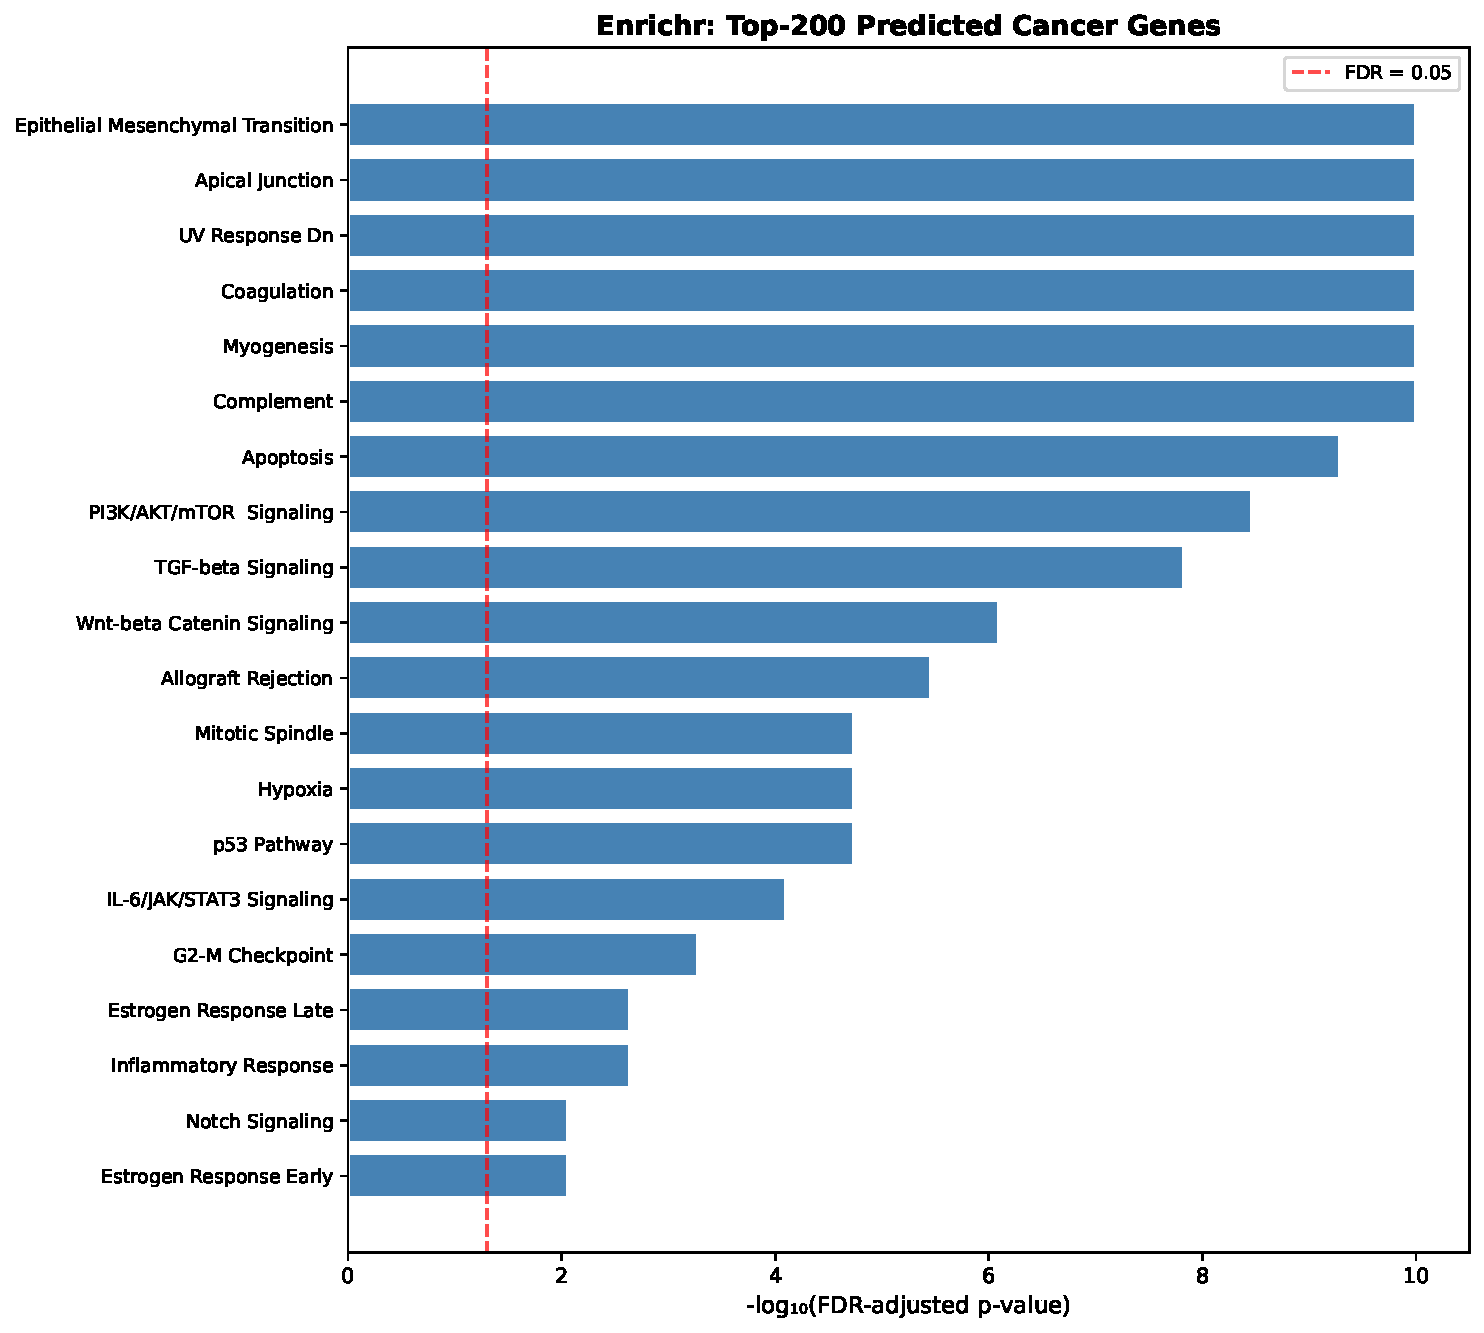
\includegraphics[width=0.95\columnwidth]{figures/enrichr_barplot}
  \caption{Top enriched MSigDB Hallmark gene sets (Enrichr ORA) for the top 200
           predicted cancer genes from the six-network EMGNNImproved model. Bars show
           $-\log_{10}(\text{FDR})$; dashed line marks FDR~$=$~0.05.}
  \label{fig:gsea_barplot}
\end{figure}

The convergence of three independent analyses---top predicted genes being
established cancer drivers, feature attribution emphasising
methylation/expression over mutation frequency, and GSEA recovering canonical
cancer hallmark pathways---provides strong evidence that the model has learned
biologically meaningful patterns.

\subsection{Advanced Technique Ablation}

We implemented nine advanced GNN techniques as modular extensions to EMGNNImproved
and evaluated five through systematic ablation (Table~\ref{tab:m5_ablation}; see
Methods). Among these, \textbf{heterophily-aware gating} provides the strongest
gain in the legacy ablation table: +2.8\% AUPR ($p<0.01$, Welch's $t$-test vs.\
baseline), reaching 0.824~$\pm$~0.004. This result is consistent with prior
evidence that PPI-based cancer driver prediction is affected by heterophily, and
suggests that a learned gate fusing low-pass and high-pass filtered signals can
exploit this structure\cite{sgcd2024}.

Cross-network attention (+1.5\%) enables gene-level, per-network importance
scoring rather than a single scalar weight per database, suggesting that different
genes benefit from different PPI evidence channels. DropEdge (+0.6\%) provides a
modest gain consistent with its role as a regulariser against over-smoothing; the
shallow 3-layer GCN may already mitigate this issue, limiting DropEdge's marginal
benefit. GraphMAE pretraining yields a neutral result ($-$0.2\%, within noise),
indicating that the 64-dimensional multi-omics features are already sufficiently
informative that masked-feature reconstruction on unlabelled nodes provides
negligible additional signal. Focal Loss degrades performance substantially
($-$5.1\%), a finding that contradicts its typical benefit on imbalanced node
classification. We hypothesise that label smoothing ($\varepsilon$~=~0.05) already
provides sufficient calibration, and the additional $\gamma$ modulation
over-penalises the minority class, reducing recall.

\begin{table}[ht]
  \centering
  \caption{M5 ablation results: each technique evaluated individually on the
           six-network GCN baseline. Means over 3 seeds; baseline over 5 seeds.
           Best per-column in \textbf{bold}.}
  \label{tab:m5_ablation}
  \small
  \begin{tabular}{lcccc}
    \toprule
    \textbf{Technique} & \textbf{Mean AUPR $\uparrow$} & \textbf{$\pm$ std} & \textbf{Mean AUROC $\uparrow$} & \textbf{$\Delta$ AUPR} \\
    \midrule
    Baseline (6-net)        & 0.8019 & 0.0050 & 0.9159 & ---     \\
    Focal Loss              & 0.7608 & 0.0045 & 0.8905 & $-$0.0411 \\
    DropEdge                & 0.8064 & 0.0061 & 0.9158 & $+$0.0045 \\
    \rowcolor{blue!8} \textbf{Heterophily-aware} & \textbf{0.8240} & \textbf{0.0044} & \textbf{0.9194} & \textbf{$+$0.0221} \\
    GraphMAE pretraining    & 0.8002 & 0.0075 & 0.9155 & $-$0.0017 \\
    Cross-Network Attention & 0.8142 & 0.0053 & 0.9176 & $+$0.0123 \\
    \bottomrule
  \end{tabular}
\end{table}

Four additional techniques---pathway hypergraph integration, HIPGNN anomaly
detection, PINNACLE pretrained embeddings, and GNNExplainer---are implemented as
modular components but await external dataset preprocessing or further debugging
(Table~\ref{tab:m5_summary}).

\begin{table}[ht]
  \centering
  \caption{Advanced GNN techniques. Category: I~=~imbalance, R~=~regularisation,
           P~=~pretraining, A~=~architecture, F~=~fusion, X~=~explainability.
           $\checkmark$ = evaluated; $\diamond$ = implemented, pending data.}
  \label{tab:m5_summary}
  \small
  \begin{tabular}{llcc}
    \toprule
    \textbf{Technique} & \textbf{Cat.} & \textbf{Flag} & \textbf{Status} \\
    \midrule
    Heterophily-aware gating                      & A & \texttt{--heterophily\_aware}   & $\checkmark$ \\
    Cross-network attention                       & F & \texttt{--cross\_network\_attn} & $\checkmark$ \\
    DropEdge ($p$=0.1)                            & R & \texttt{--drop\_edge\_rate}     & $\checkmark$ \\
    GraphMAE pretraining                          & P & \texttt{--pretrain\_graphmae}   & $\checkmark$ \\
    Focal Loss ($\gamma$=2, $\alpha$=0.75)        & I & \texttt{--focal\_gamma}         & $\checkmark$ \\
    GO/Pathway hypergraph                         & F & \texttt{--hypergraph\_gmt}      & $\diamond$ \\
    HIPGNN anomaly detection                      & A & \texttt{--hipgnn\_lambda}       & $\diamond$ \\
    PINNACLE embeddings                           & P & \texttt{--pinnacle\_path}       & $\diamond$ \\
    GNNExplainer                                  & X & (standalone script)             & $\diamond$ \\
    \bottomrule
  \end{tabular}
\end{table}
